\section{Experimental Design}
\label{sec:experimental_design}

\begin{figure*}[!t]
\centering
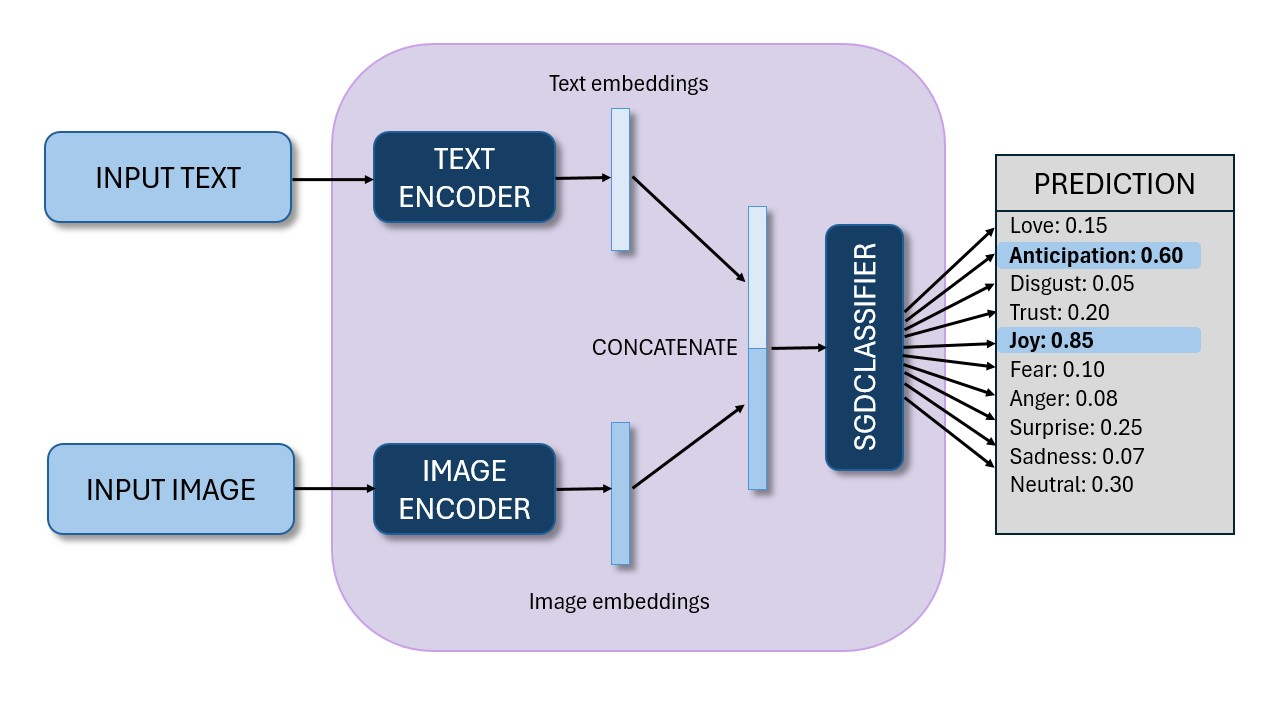
\includegraphics[width=0.78\textwidth]{imgs/model_architecture.jpeg}
\caption{Dual-Encoder multimodal architecture. Text and image representations are extracted in parallel via domain-adapted BERT and ViT encoders, concatenated into a joint vector ($d=1536$), and passed to a Classifier Chain head.}
\label{fig:dual_encoder_arch}
\end{figure*}

This section details the experimental methodology established to evaluate affective classification on the MultiEMiT corpus. We evaluate three distinct tasks: Emotion Detection, Irony Detection, and Semiotic Relation Detection. The experiments measure the performance differences between unimodal textual baselines, a discriminative multimodal architecture (Dual-Encoder), and a generative foundation model (Pixtral 12B), while assessing the empirical impact of correlation prompting across architectures.

We formalize three classification benchmarks corresponding to different levels of communicative intent:
\begin{itemize}\setlength{\itemsep}{1pt}\setlength{\parskip}{0pt}\setlength{\topsep}{2pt}
    \item \textbf{Emotion Detection:} Multi-label classification over ten candidate emotions (\textit{Anger}, \textit{Anticipation}, \textit{Disgust}, \textit{Fear}, \textit{Joy}, \textit{Love}, \textit{Neutral}, \textit{Sadness}, \textit{Surprise}, and \textit{Trust}). Models predict any valid subset of concurrent emotions using binary cross-entropy or binary chains.
    \item \textbf{Irony Detection:} Single-label classification categorizing each post into one of three mutually exclusive classes: \textit{Unironic}, \textit{Irony}, or \textit{Sarcasm}.
    \item \textbf{Semiotic Relation Detection:} Single-label classification identifying the semantic text--image interaction as \textit{Additive}, \textit{Parallel}, or \textit{Divergent}.
\end{itemize}

Due to heavy class skew, raw accuracy paints a misleading picture of model quality. We therefore evaluate systems using \textbf{Precision}, \textbf{Recall}, and the \textbf{F1-score}. In overall comparisons across all three tasks, the \textbf{Macro F1-score} serves as the primary metric, weighting each class equally to penalize poor performance on minority labels. In fine-grained subset evaluations across semiotic relations (Section~\ref{sec:results}), we report the \textbf{Micro F1-score} to maintain metric stability when sample sizes in individual subsets are small.

To establish strong text-only reference points, we evaluated models built on the RoBERTa architecture. For Irony and Semiotic Relation detection, we used \textit{UmBERTo} \cite{musixmatch-2020-umberto}, a RoBERTa-based language model pre-trained on Italian Common Crawl with whole-word masking. For Irony detection, UmBERTo was first fine-tuned on the IronITA benchmark \cite{ironita2018} before adaptation to MultiEMiT. For Emotion Detection, we used \textit{FEEL-IT} \cite{bianchi2021feel}, fine-tuned on the combined MultiEMiT textual split and the external EMiT dataset \cite{emit} to adapt its representation space to our ten-class taxonomy. These text models process the tweet text alone without visual inputs.

To capture cross-modal interactions, we implemented a discriminative Dual-Encoder pipeline (Fig.~\ref{fig:dual_encoder_arch}). 
The textual modality is processed by the domain-adapted language encoder (FEEL-IT for emotions, UmBERTo for irony and relations), while the visual modality is processed in parallel by a Vision Transformer (ViT-base-patch16-224) \cite{dosovitskiy2021vit}.
Both unimodal encoders extract high-level representations: the 768-dimensional `[CLS]` token embedding from the text transformer and the 768-dimensional pooled representation from the ViT are concatenated into a 1536-dimensional joint multimodal vector.

To predict class labels from this joint representation, we employ Classifier Chains \cite{pedregosa2011scikit}. This architecture models label interdependencies by sequentially conditioning subsequent binary classifiers on previous predictions, making it well suited for multi-label emotion spaces. Specifically, we configure Scikit-Learn's \texttt{ClassifierChain} wrapping an \texttt{SGDClassifier} with logistic loss, $L_2$ regularization, and fixed random seeding. This linear head projects the concatenated latent space to class predictions without overfitting on the compact multimodal split.

Motivated by the strong label dependencies discovered during corpus analysis (Section~\ref{sec:dataset_analysis}), we developed a structured \textit{Correlation Prompting} strategy. Rather than hoping the neural network will infer subtle cross-task correlations from scarce training examples, we inject empirical Pearson correlation coefficients directly into the input text as natural language context. For example, in the Irony detection task, the input tweet is appended with: \textit{``Statistics: Sarcasm correlates positively with Disgust and Anger. Irony correlates positively with Divergent relation.''}

To evaluate model sensitivity to the volume of injected priors, we structured prompts across three distinct correlation tiers based on Pearson coefficient thresholds: (i) \textbf{Short prompts}, incorporating only strong associations with $|r| \ge 0.25$; (ii) \textbf{Medium prompts}, including moderate correlations with $|r| \ge 0.20$; and (iii) \textbf{Long prompts}, providing detailed contextual priors with all correlations satisfying $|r| \ge 0.15$. All prompt instructions were formulated in English, following findings from the BRIGHTER benchmark \cite{brighter_project} indicating that multilingual LLMs adhere better to instructions and exhibit lower variance when prompted in English rather than the target language.

To compare specialized discriminative systems against modern generative vision-language models, we benchmarked \textbf{Pixtral 12B} \cite{pixtral}, an open-weights multimodal language model based on Mistral Nemo featuring a dedicated 400M-parameter vision encoder capable of handling arbitrary image resolutions.
We evaluated Pixtral across three experimental regimes:
\begin{itemize}\setlength{\itemsep}{1pt}\setlength{\parskip}{0pt}\setlength{\topsep}{2pt}
    \item \textbf{Zero-Shot Prompting:} Out-of-the-box reasoning across prompt tiers (Short, Medium, and three Long prompt formulations: \textit{long\_v1}, \textit{long\_v2}, \textit{long\_v3}), testing generation with and without correlation context.
    \item \textbf{Few-Shot (Three-Shot) Prompting:} In-context learning for Semiotic Relation Detection, providing three complete multimodal exemplars (one per relation category) within the prompt window.
    \item \textbf{LoRA Fine-Tuning:} Low-Rank Adaptation on the MultiEMiT multimodal training set ($r=16$, $\alpha=32$, RSLoRA, all linear target modules, dropout $0.1$). This configuration adapts 66,322,432 parameters out of 12.75 billion (0.52\% trainable parameters). Training ran with per-device batch size 1, 8 gradient accumulation steps (effective batch size 8), learning rate $3 \times 10^{-5}$, FP16 mixed precision, and gradient checkpointing over 2 epochs.
\end{itemize}

All generative experiments were evaluated over three independent runs at two decoding temperatures: $T=0.1$ (greedy, low-variance decoding) and $T=0.9$ (stochastic exploratory decoding).

Unlike discriminative encoders that output bounded probability vectors over predefined classes, Pixtral generates labels autoregressively. During multi-label emotion fine-tuning, ranking bias and exposure bias degraded the stopping token (\texttt{<EOS>}), causing repetitive token loops and out-of-vocabulary synonyms (e.g., generating \textit{Joy, Joy, Happiness} instead of \textit{Joy}). To resolve this without retraining, we implemented a post-processing truncation parameter $n$, restricting extraction to the first $n$ unique valid taxonomy emotions generated. Setting $n=2$ matches the empirical ground truth and eliminates unconstrained tail hallucinations.
